\documentclass[14pt,a4paper,bach]{dipNSU}%загрузка класса. базовый класс -- extreport 
%magis -- для магистратуры bach -- для бакалавриата
\usepackage{amsmath,amssymb,amsfonts}%математика
\usepackage{xcolor}%цвета
\usepackage{lipsum} % for dummy text only
\usepackage[colorlinks = true,
linkcolor = red,
urlcolor  = blue,
citecolor = blue,
anchorcolor = blue]{hyperref}% \href ссылки

\usepackage{setspace}%установка межстрочного интервала
\usepackage{tabularx}%окружение таблиц tabularx
\usepackage{multirow} %объединение строк в таблицах
\usepackage{booktabs}%для всяких украшательств в таблицах (\toprule,\midrule ...)
\usepackage{float} %работа с ``плавающими'' объектами [H]
\usepackage{graphicx}% графика
\usepackage{wrapfig}%картинки с обтеканием

\usepackage{minted}%листинг кода

%мощный пакет для построения графики разной степени сложности. В обычных текстах обычно не нужен
\usepackage{tikz}
\usepackage{smartdiagram}
\usetikzlibrary{positioning}
\usetikzlibrary{decorations} 
\usetikzlibrary{shapes,arrows}
\usepgflibrary{arrows.meta}
\usetikzlibrary{arrows.meta}
\usetikzlibrary{bending}
\usetikzlibrary{graphs}
\usetikzlibrary{decorations.pathmorphing}
\usetikzlibrary{calc,patterns,angles,quotes}

%вставить список используемых дополнительных пакетов
\graphicspath{{figures/}}% путь к рисункам относительно данного документа

\UpperOrganization{МИНИСТЕРСТВО НАУКИ И ВЫСШЕГО ОБРАЗОВАНИЯ РОССИЙСКОЙ~ФЕДЕРАЦИИ}%минобр
\OrganizationType{ФЕДЕРАЛЬНОЕ ГОСУДАРСТВЕННОЕ АВТОНОМНОЕ ОБРАЗОВАТЕЛЬНОЕ УЧРЕЖДЕНИЕ ВЫСШЕГО ОБРАЗОВАНИЯ}%тип организации
\Organization{<<НОВОСИБИРСКИЙ НАЦИОНАЛЬНЫЙ ИССЛЕДОВАТЕЛЬСКИЙ ГОСУДАРСТВЕННЫЙ УНИВЕРСИТЕТ>> (НОВОСИБИРСКИЙ ГОСУДАРСТВЕННЫЙ УНИВЕРСИТЕТ, НГУ)}%полное название университета
\Faculty{ФИЗИЧЕСКИЙ}%название факультета
\Department{ФИЗИКИ ПЛАЗМЫ}%название кафедры


\title{Шаблон выпускной квалификационной работы}%заголовок курсовой
\author{Анненкова Владимира Вадимовича}%ФИО автора в родительном падеже полностью


\Superviser{ФИО руководителя}%руководитель
\SuperviserDegree{д.ф.-м.н., профессор}%учёная степень руководителя
\SuperviserWorkPlace{г.н.с., ИЯФ СО РАН}%должность и место работы руководителя

\DepHead{Беклемишев А.Д.}%зав.каф.
\DepHeadDegree{к.ф.-м.н.}%учёная степень
\DepHeadWorkPlace{в.н.с., ИЯФ СО РАН}%должность и место работы зав.кафа.




\KeyWords{Физика плазмы, численное моделирование, \LaTeXe}%ключевые слова


\RefSource{ref}%название файла с библиографией
\SetPDFmeta%установить метаданные pdf файла

%\makeatletter
%\newcommand\thefontsize[1]{{#1 The current font size is: \f@size pt\par}}
%\makeatother


\begin{document}
\maketitle%Создать титульный лист


%команда \input вставляет заместо себя содержимое указанного файла


{
	\hypersetup{linkcolor=black}%чёрный цвет текста
	\tableofcontents%Сгенерировать оглавление
}

%\Definitions%определения, используемые в работе. Формально в ГОСТе такой пункт есть, реально в курсовой его использовать особого смысла нет
\Introduction

Это шаблон ВКР, разработанный на основе требований  ГОСТ и деканата \href{http://www.phys.nsu.ru/department/index.php/diplomnikam}{http://www.phys.nsu.ru/department/index.php/diplomnikam}

Также в данном шаблоне содержится некоторое количество примеров  использования \LaTeX'а при вёрстке текста и ссылки на различные полезные источники.

%Введение	
\chapter{Основная часть}\label{ch:ch1}

Пример главы%глава основной части
\chapter{Об этом шаблоне}\label{ch:about}




Данный шаблон создан на основе \href{https://docs.cntd.ru/document/1200026224}{ГОСТ 7.32-2001} ''Отчет о научно-иссле\-до\-ва\-тельской работе. Структура и правила оформления'' и рекомендаций деканата ФФ НГУ:

\href{http://www.phys.nsu.ru/main/index.php/main/news/652-2016-03-01-news-kursovye}{\small http://www.phys.nsu.ru/main/index.php/main/news/652-2016-03-01-news-kursovye}

Настоятельно рекомендуется ознакомиться с этими двумя ресурсами.

Шаблон предназначен для вёрстки посредством \verb*|pdflatex| или \verb*|xelatex| и \verb*|bibtex| (библиография)

Необходимые файлы шаблона:
\begin{enumerate}
	\item \verb*|kurs3.cls| --- настройки класса: объявление вспомогательных команд, настройка оформления и титульного листа;
	\item \verb*|Preamble.tex| --- файл с перечислением подключаемых пакетов;
	\item \verb*|ugost2008.bst| --- стилевой пакет библиографии по ГОСТу 7.0.5-2008. Необходим при вёрстке на локальном ПК --- при использовании \href{https://www.overleaf.com}{overleaf} не нужен. Он там есть по-умолчанию.
	\item \verb*|kurs3temp.tex| --- основной документ, в который подключаются остальные файлы и сам текст;
	\item  \verb*|ref.bib| --- файл с библиографией в формате \verb*|bibtex|'а.
\end{enumerate}

При вёрстке \verb*|pdflatex|'ом шаблон по-умолчанию использует шрифт с засечками Computer Modern Roman (CMR). Это не Times New Roman (TMN) (проприетарный шрифт), который указывается в различных требованиях и ГОСТах. Отдельный вопрос почему он там указывается. Скорее всего фактически имелся ввиду ''шрифт с засечками''. Во времена написания требований офисный документооборот осуществлялся с помощью ПО Microsoft, в котором этот шрифт был основным шрифтом с засечками. На практике проблем с использованием CMR обычно не бывает (особенно в курсовых работах).

Если всенепременно хотите использовать TMN, то есть два пути:

\begin{enumerate}
	\item Если использовать \verb*|pdflatex|, то нужно в файле  \verb*|kurs3.cls| раскомментировать строки
	
	\verb*|\RequirePackage[math]{pscyr}|
	
	\verb*|\renewcommand{\rmdefault}{ftm}|
	
	Это включит использование пакета \verb*|pscyr|, который предварительно нужно установить на Вашу ОС. Этот пакет предоставляет также другие интересные шрифты, например шрифт ''как в старых учебниках'':
	
	 \verb*|\renewcommand{\rmdefault}{fac}|
	\item \verb*|xelatex| позволяет использовать в \verb|.tex| документах системные шрифты. Шаблон настроен таким образом, что при вёрстке им автоматически будет выбрано использование системного шрифта TNR (он должен быть установлен!).
\end{enumerate}

Также этот шаблон успешно верстается в онлайн системе overleaf (кроме режима с использованием pscyr). 

\newpage
Список команд, введёных в данном шаблоне и не являющихся стандартными для \LaTeX:
\begin{enumerate}
	\small
	\setlength\itemsep{-0.3cm}
	\item \verb*|\SetPDFmeta| --- установка метаданных pdf документа
	\item \verb*|\Organization| --- переменная для хранения названия организации
	\item \verb*|\OrganizationType| --- тип организации
	\item \verb*|\UpperOrganization| --- вышестоящая организация
	\item \verb*|\Faculty| --- название факультета
	\item \verb*|\Department| --- название каферды
	\item \verb*|\Superviser| --- фамилия и инициалы руководителя
	\item \verb*|\SuperviserDegree| --- учёная степень и звание (если есть) руководителя
	\item \verb*|\SuperviserWorkPlace| --- должность и место работы руководителя
	\item \verb*|\DepHead|  --- фамилия и инициалы зав. кафа
	\item \verb*|\DepHeadDegree| --- учёная степень и звание (если есть) зав. кафа
	\item \verb*|\DepHeadWorkPlace| --- должность и место работы зав. кафа
	\item \verb*|\RefSource| --- название файла с библиографией
	\item \verb*|\ChapterWithoutNum| --- вспомогательная команда для форматирования заголовка раздела без номера (Введение и т.п.)
	\item \verb*|\References| --- создания списка литературы
	\item \verb*|\Definitions| --- заголовок Определения с добавлением в оглавление без номера
	\item \verb*|\Abbreviations| --- заголовок Сокращения и обозначения с добавлением в оглавление без номера
	\item \verb*|\Introduction| --- заголовок Введение с добавлением в оглавление без номера
	\item \verb*|\Conclusion| --- заголовок Заключение с добавлением в оглавление без номера
	\item \verb*|\Appendix| --- заголовок Приложение с добавлением в оглавление без номера, с увеличением счётчика
\end{enumerate}%об этом шаблоне
%главы с примерами использования LaTeX'а
%заместо этих и других глав ставьте свои
\chapter{\LaTeX}\label{ch:latex}

\section{Установка}


\begin{itemize}
	\setlength{\itemsep}{1pt}%регулировка расстояния между элементами
	\setlength{\parskip}{1pt}%
	\item Windows: TeX Live \href{https://www.tug.org/texlive/acquire-netinstall.html}{https://www.tug.org/texlive/acquire-netinstall.html}
	\item Linux: пакет texlive-full\footnote{Это пример сноски, генерируемой командой \mintinline{tex}{\footnote{...}}| }
	\item Пример IDE: \href{https://www.texstudio.org/}{https://www.texstudio.org/}
	\item Бесплатная онлайн система вёрстки: \href{https://www.overleaf.com/}{https://www.overleaf.com/}
\end{itemize}

\section{Учебные материалы}

\begin{itemize}
	\item Большой проект на русском с самых основ (слегка устарел в плане рекомендуемого ПО, но информация по \LaTeX'у актуальна):
	
	 \href{http://mydebianblog.blogspot.com/2008/11/latex.html}{http://mydebianblog.blogspot.com/2008/11/latex.html}
	 \item Много гайдов: \href{https://www.overleaf.com/learn}{https://www.overleaf.com/learn}
	\item \href{http://www.inp.nsk.su/~baldin/LaTeX/}{http://www.inp.nsk.su/\textasciitilde baldin/LaTeX/}
	\item Литература:
	\begin{itemize}
		\item Котельников И.А., Чеботаев П.З., \textit{LaTeX по-русски }
		
		\href{https://www.researchgate.net/publication/235255954_LaTeX_po-russki}{\small https://www.researchgate.net/publication/235255954\_LaTeX\_po-russki}
		
		\item Львовский С. М., \textit{Набор и вёрстка в системе \LaTeX}
		
		 \href{https://www.mccme.ru/free-books/llang/newllang.pdf}{\small https://www.mccme.ru/free-books/llang/newllang.pdf}
	\end{itemize}
\end{itemize}

\section{Презентации и постеры}

С помощью \LaTeX также можно оформлять презентации и постеры. Особенно удобно это для тех, у кого в работе много формул. Удобнее всего это делать с помощью пакета \verb*|beamer|. Набор материалов по нему:
\begin{itemize}
	\item Официальная документация:
	
	 \href{http://tug.ctan.org/macros/latex/contrib/beamer/doc/beameruserguide.pdf}{\small http://tug.ctan.org/macros/latex/contrib/beamer/doc/beameruserguide.pdf} 
	 \item На overleaf:
	 
	 Туториал для новичков: \href{https://www.overleaf.com/learn/latex/Beamer_Presentations:_A_Tutorial_for_Beginners_(Part_1)%E2%80%94Getting_Started}{ссылка} 
	 	
	 \href{https://www.overleaf.com/learn/latex/beamer}{https://www.overleaf.com/learn/latex/beamer}
	 \item На русском языке:
	  
	  \href{https://proft.me/2014/05/31/beamer-kachestvennaya-prezentaciya-sredstvami-late/}{\small https://proft.me/2014/05/31/beamer-kachestvennaya-prezentaciya-sredstvami-late/}
	  
	  \href{https://habr.com/ru/post/145523/}{https://habr.com/ru/post/145523/}
	  \item Про постеры:
	  
	  \href{http://mydebianblog.blogspot.com/2010/12/beamerposter.html}{http://mydebianblog.blogspot.com/2010/12/beamerposter.html}
	  
	  \href{https://www.overleaf.com/gallery/tagged/poster}{https://www.overleaf.com/gallery/tagged/poster}
	  
	  Но для постеров возможно удобнее сразу использовать пакет Tikz:
	  
	  \href{https://ru.overleaf.com/learn/latex/Posters}{https://ru.overleaf.com/learn/latex/Posters}
\end{itemize}


\section{Начертания шрифтов}
\noindent%выключить красную строку
\textnormal{(Default) Основной шрифт документа}\\
\textrm{(Roman) С засечками}\\
\textit{(Italic) Курсив — не наклонный!}\\
\textsl{(Slanted) Наклонный — не курсив!}\\
\textbf{(Bold) Жирный}\\
\textbf{\textit{(Bold italic) Жирный курсив}}\\
\textbf{\textsl{(Bold slanted) Жирный наклонный}}\\
\texttt{(Monospace) Моноширинный}\\
\textsc{(Small caps) «Малые заглавные»}\\
\textbf{\textsc{(Bold Small caps) Жирный «Малые заглавные»}}\\
\textsf{(Sans serif) без засечек}

\section{Размеры шрифтов}\label{sec:font_size}

\begin{tabular}{cl}
	\hline
\tiny{Текст}	& \verb*|\tiny{Текст}| \\
\scriptsize{Текст}& \verb*|\scriptsize{Текст}| \\
\footnotesize{Текст}& \verb*|\footnotesize{Текст}| \\
\small{Текст}& \verb*|\small{Текст}| \\
\normalsize{Текст}& \verb*|\normalsize{Текст}| \\
\large{Текст}& \verb*|\large{Текст}| \\
\Large{Текст}& \verb*|\Large{Текст}| \\
\LARGE{Текст}& \verb*|\LARGE{Текст}| \\
\huge{Текст}& \verb*|\huge{Текст}| \\
\Huge{Текст}& \verb*|\Huge{Текст}| \\
\hline
\end{tabular}


\section{Ссылки на элементы документа}


Для того, что бы ссылаться на объект документа (главу, таблицу, рисунок, формулу и т.д.) сперва нужно повесить на него ярлык, т.е. прописать рядом с ним \verb*|\label{название_ссылки}|. Затем в любом месте текста на неё можно ссылаться с помощью команды: \verb*|\ref{название_ссылки}|

Примеры:

Изменение размеров шрифтов продемонстрировано в разделе~\ref{sec:font_size}. В Главе~\ref{ch:tab} обсуждается создание таблиц. Рисунок~\ref{fig:image1}~--- это первый рисунок в данном документе. А вот ссылка на Таблицу~\ref{tab:GOST1}.

Для того, чтобы в итоговом документе появились ссылки необходимо собрать его дважды.

\section{Правила русской типографии}

Желающим готовить качественные тексты настоятельно рекомендую ознакомиться с основными правилами русской типографии:

\begin{itemize}
	\item \href{https://habr.com/ru/post/75662/}{https://habr.com/ru/post/75662/}
	\item \href{https://ivgpu.com/images/docs/sotrudniku/rabota-s-sajtom/pravila-tipografiki.pdf}{\small https://ivgpu.com/images/docs/sotrudniku/rabota-s-sajtom/pravila-tipografiki.pdf}
	\item \href{https://ru.wikibooks.org/wiki/LaTeX/%D0%A4%D0%BE%D1%80%D0%BC%D0%B0%D1%82%D0%B8%D1%80%D0%BE%D0%B2%D0%B0%D0%BD%D0%B8%D0%B5_%D1%82%D0%B5%D0%BA%D1%81%D1%82%D0%B0}{https://ru.wikibooks.org/wiki/LaTeX/Форматирование\_текста}
\end{itemize}


\chapter{Списки}
\section{Ненумерованный}
\begin{itemize}
	\item раз
	\item два
	\item Список второго уровня
	\begin{itemize}
		\item три
		\item четыре
		\item пять
	\end{itemize}
\end{itemize}


Список с изменённым расстоянием между элементами с помощью команды \verb*|\setlength\itemsep{-0.2cm}| 
\begin{itemize}
	 \setlength\itemsep{-0.2cm}
	\item раз
	\item два
	\item Список второго уровня
\end{itemize}
Лучше в тексте не используйте без очень большой надобности.

\section{Нумерованный}
\begin{enumerate}
	\item раз
	\item два
	\item Список второго уровня
	\begin{enumerate}
		\item три
		\item четыре
		\item пять
	\end{enumerate}
\end{enumerate}
\chapter{Таблицы}\label{ch:tab}
\begin{itemize}
	\item 	\href{http://mydebianblog.blogspot.com/2009/01/tables-in-latex.html}{http://mydebianblog.blogspot.com/2009/01/tables-in-latex.html}
	
	\item 	\href{http://mydebianblog.blogspot.com/2013/01/advanced-tables-in-latex.html}{http://mydebianblog.blogspot.com/2013/01/advanced-tables-in-latex.html} 
\end{itemize}

Для некоторых приведённых примеров требуются пакеты:

окружение таблиц tabularx:\verb|\usepackage{tabularx}|

объединение строк в таблицах:
\verb|\usepackage{multirow}|

для всяких украшательств в таблицах:
\verb|\usepackage{booktabs}|

работа с ``плавающими'' объектами:
\verb|\usepackage{float}|


По ГОСТу оформлены таблицы \ref{tab:GOST1} и \ref{tab:GOST2}.


\begin{table}[ht]
	%\renewcommand{\arraystretch}{1.8} %% increase table row spacing
	%\renewcommand{\tabcolsep}{1cm}   %% increase table column spacing
	\caption{Простая таблица}
	\begin{tabular}{|c|c|r|l|}
		\hline
		раз & два & три & четыре \\
		\hline
		1 & 2 & 3 & 4 \\
		\hline
		пять & шесть & семь & восемь \\
		\hline
		9 & 10 & 11 & 12 \\
		\hline
	\end{tabular}
\end{table}


\begin{table}[H]
		\caption{Такая таблица по ГОСТу}
		\label{tab:GOST1}
	\begin{center}
		\begin{tabular}{|c|c|c|}
			\hline
			\multirow{3}{*}{Размеры нестандартных болтов} & \multicolumn{2}{c|}{Диаметр} \\
			\cline{2-3}
			& Норма & Разброс \\
			\cline{2-3}
			& 10 мм & 1 мм \\
			\hline
		\end{tabular}
	\end{center}
\end{table}

\begin{table}[H]
		\caption{Такая таблица по ГОСТу}
		\label{tab:GOST2}
	\begin{center}
		\begin{tabular}{|c|c|c|}
			\hline
			& \multicolumn{2}{c|}{Диаметр} \\
			\cline{2-3}
			\raisebox{1.5ex}[0cm][0cm]{Нестандартные болты}
			& Норма & Разброс \\
			\hline
			Размеры & 10 мм & 1 мм \\
			\hline
		\end{tabular}
	\end{center}
\end{table}

\begin{table}[htbp]
	\caption{Таблица по ширине страницы}
	\begin{tabularx}{\textwidth}{XXXXX}
		\toprule
		auto & break & case & char & const\\
		%	\hline
		continue   & default   & do & double & else\\
		%	\hline
		\bottomrule
	\end{tabularx}
\end{table}

\begin{table}[htbp]
	\centering
	\caption{Изменённое соотношение ширин столбцов}
	\begin{tabularx}{.85\textwidth}{>{\hsize=0.075\textwidth}XX>{\hsize=0.075\textwidth}XX}
		\toprule
		== & Равно & != & Не равно\\
		> & Больше & < & Меньше\\
		\bottomrule
	\end{tabularx}
\end{table}


\begin{table}[!hbt]
		\caption{Таблица с фиксированной шириной колонок и увеличенным размером строк.}
	\begin{center}
		\renewcommand{\arraystretch}{1.2} %% increase table row spacing	
		\begin{tabular}{|>{\raggedright\arraybackslash}m{3.2cm}|>{\arraybackslash}p{1.9cm}|>{\raggedright\arraybackslash}m{5cm}|>{\raggedright\arraybackslash}m{5cm}|}
			\hline
			\textbf{Величина} & \textbf{Обоз-е} & \textbf{Значение в СИ} & \textbf{Значение в СГС} \\
			\hline
			\textbf{Масса электрона} & $m_e$ &$9.1094\cdot10^{-31}$, кг  & $9.1094\cdot10^{-28}$, г  \\
			\hline
			
		\end{tabular}
	\end{center}
\end{table}	
\chapter{Картинки}\label{ch:fig}

Рисунки следует готовить в хорошем качестве. Современные графические приложения как правило позволяют создавать графики в \href{https://ru.wikipedia.org/wiki/%D0%92%D0%B5%D0%BA%D1%82%D0%BE%D1%80%D0%BD%D0%B0%D1%8F_%D0%B3%D1%80%D0%B0%D1%84%D0%B8%D0%BA%D0%B0}{векторном} виде и сохранять их в формате \verb|.pdf|, которые затем можно вставлять в \LaTeX\, документы. Если готовите растровые иллюстрации, то старайтесь делать их с высоким \href{https://ru.wikipedia.org/wiki/Dots_per_inch}{DPI} (больше 150, например). Рекомендуется по возможности  использовать форматы без потери качества (например \verb|.png|).

О вставке изображений:

\begin{itemize}
	\item \href{http://mydebianblog.blogspot.com/2008/12/latex_15.html}{http://mydebianblog.blogspot.com/2008/12/latex\_15.html}
	\item \href{http://mydebianblog.blogspot.com/2013/03/amorua-advanced-floats.html}{http://mydebianblog.blogspot.com/2013/03/amorua-advanced-floats.html}
	\item \href{https://www.overleaf.com/learn/latex/Inserting_Images}{https://www.overleaf.com/learn/latex/Inserting\_Images}
	\item \href{https://www.overleaf.com/learn/latex/Positioning_of_Figures}{https://www.overleaf.com/learn/latex/Positioning\_of\_Figures}
\end{itemize}







\begin{figure}[h]
	\centering
	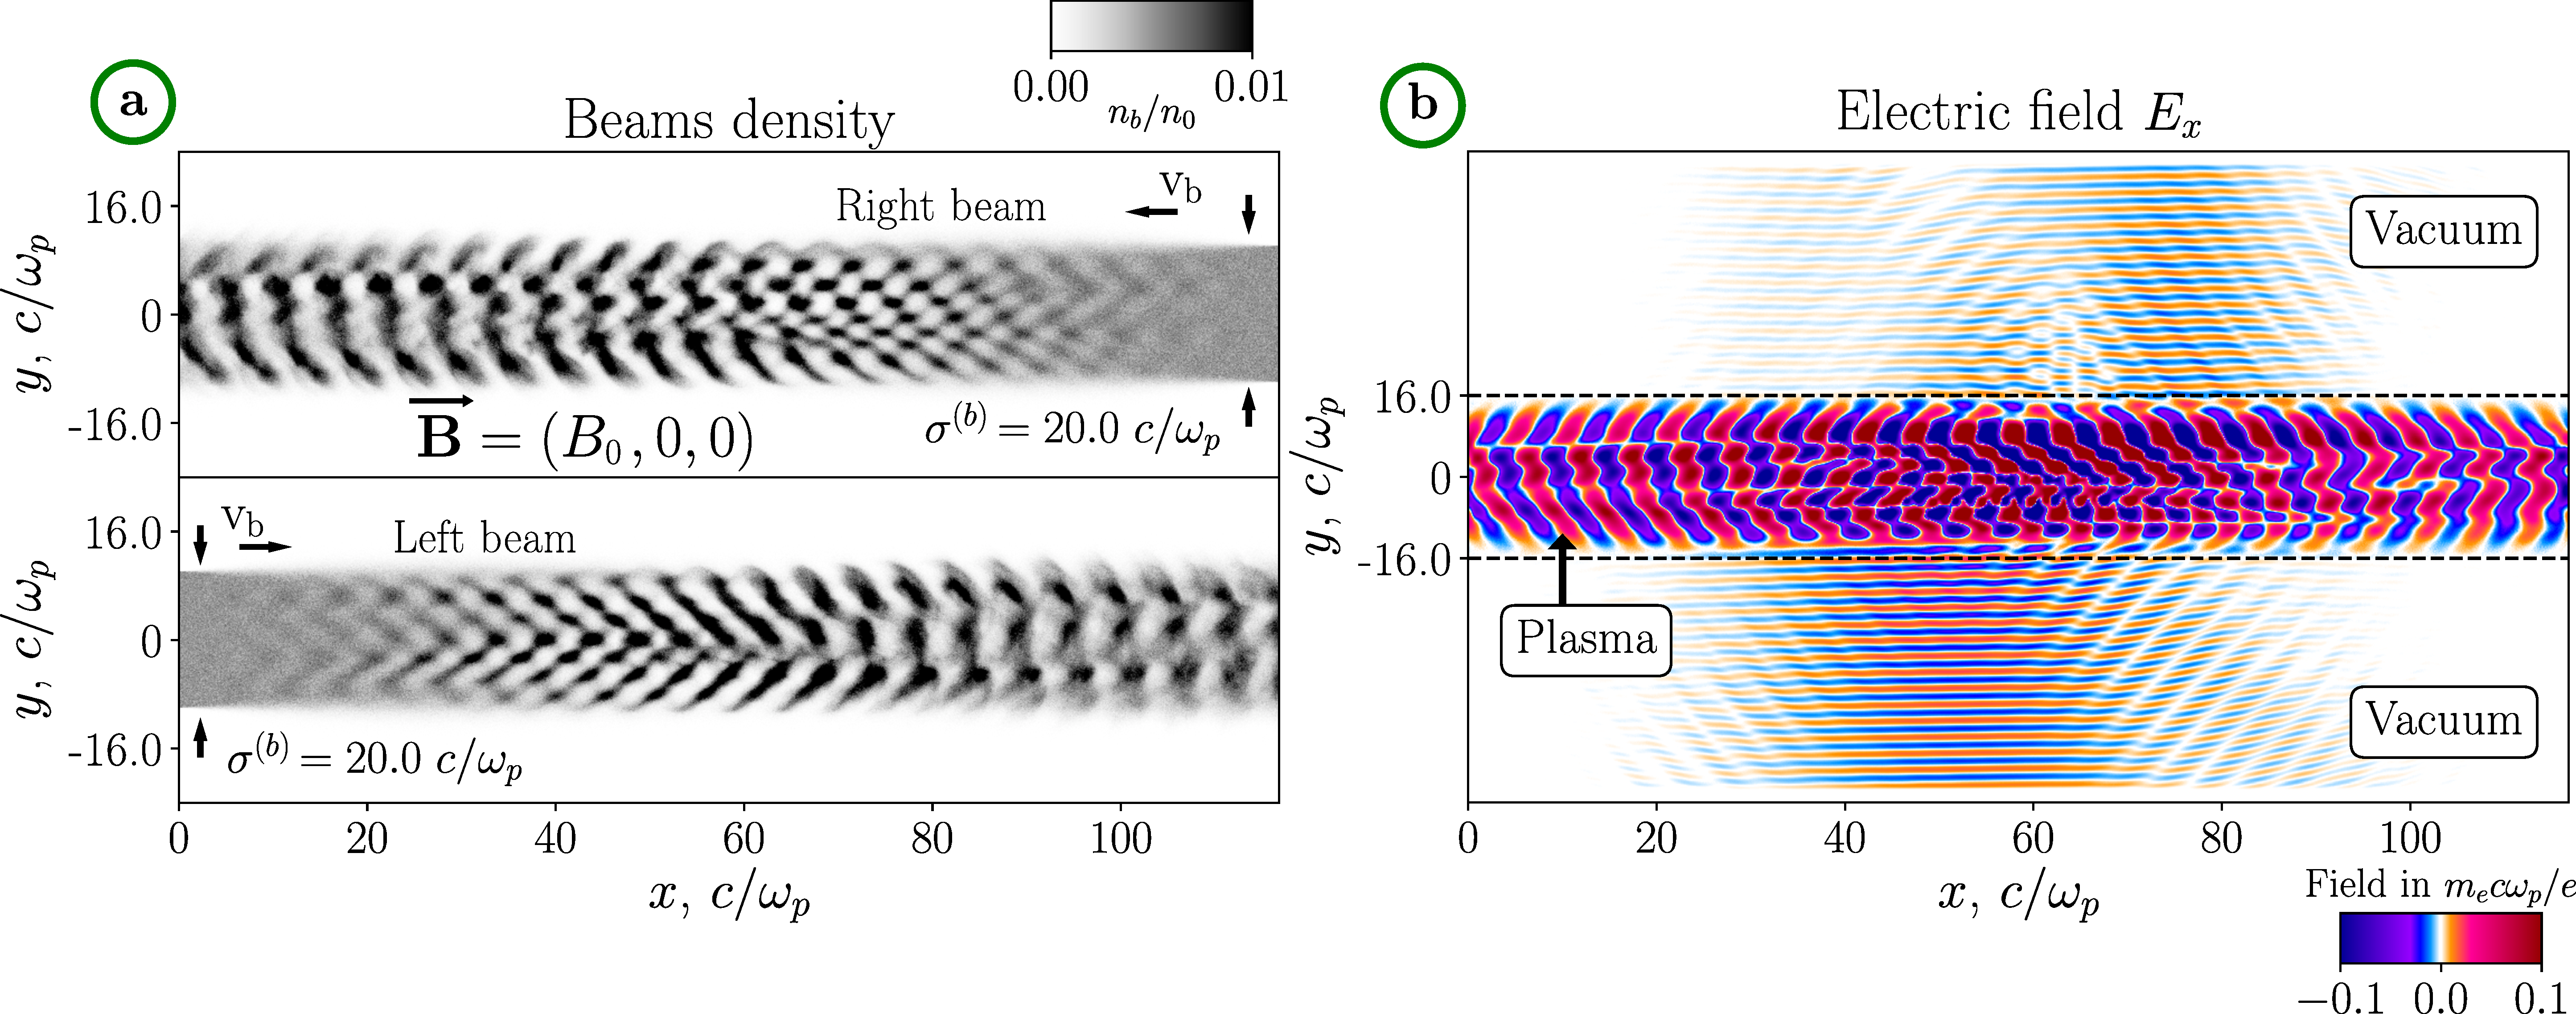
\includegraphics[width=0.95\linewidth]{fig2.pdf}
	\caption{Одна картинка по центру размером 0.95 длины строки}
	\label{fig:image1}%ссылка на картинку
\end{figure}


\begin{figure}[h]
	\begin{center}
		\begin{minipage}[h]{0.45\linewidth}
			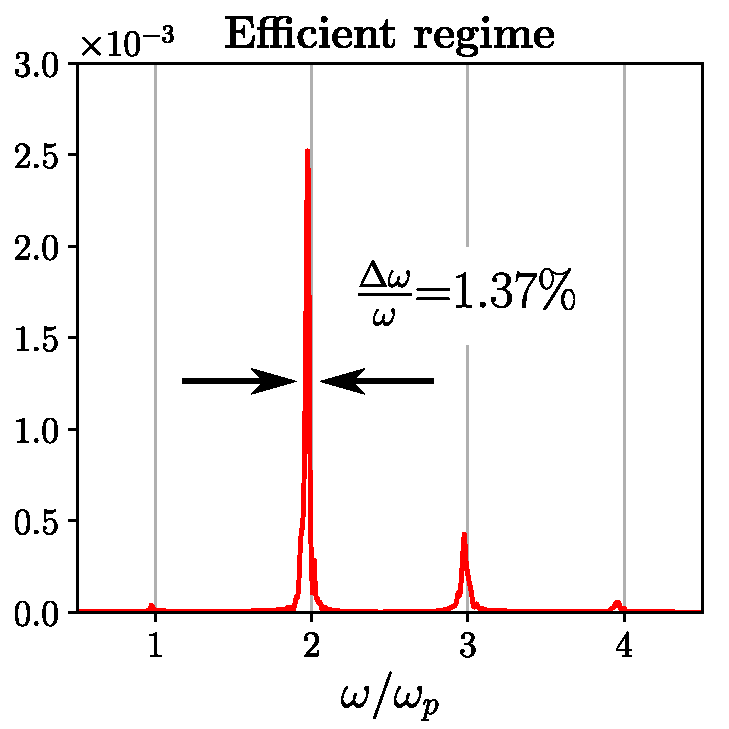
\includegraphics[width=1\linewidth]{fig09}
			\caption{Два изображения в строчку.} %% подпись к рисунку
			\label{fig:image2} %% метка рисунка для ссылки на него
		\end{minipage}
		\hfill
		\begin{minipage}[h]{0.45\linewidth}
			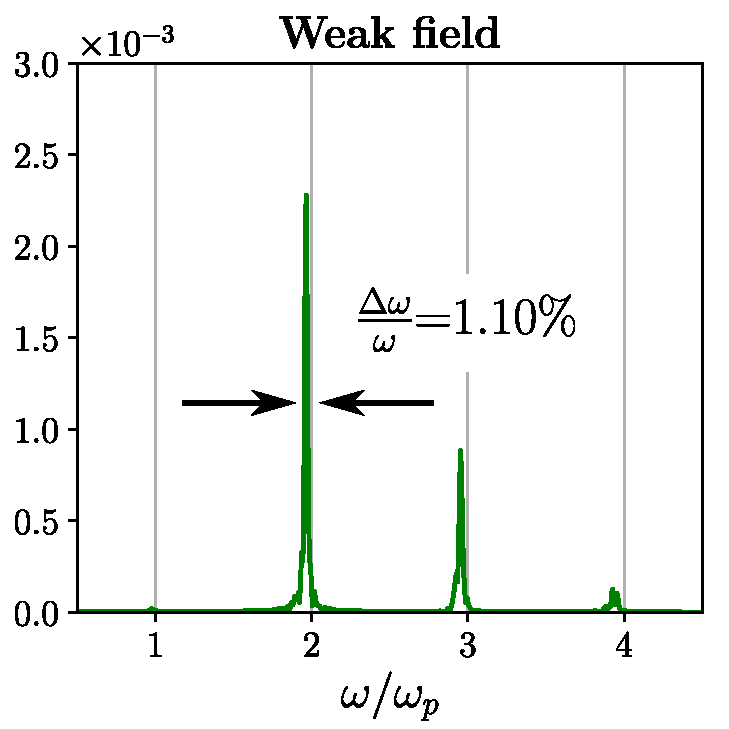
\includegraphics[width=1\linewidth]{fig10}
			\caption{С индивидуальными подписями.}
			\label{fig:image3}
		\end{minipage}
	\end{center}
\end{figure}


\section{С обтеканием}
\lipsum[1-2]

\begin{wrapfigure}[12]{r}{0.45\linewidth} 

	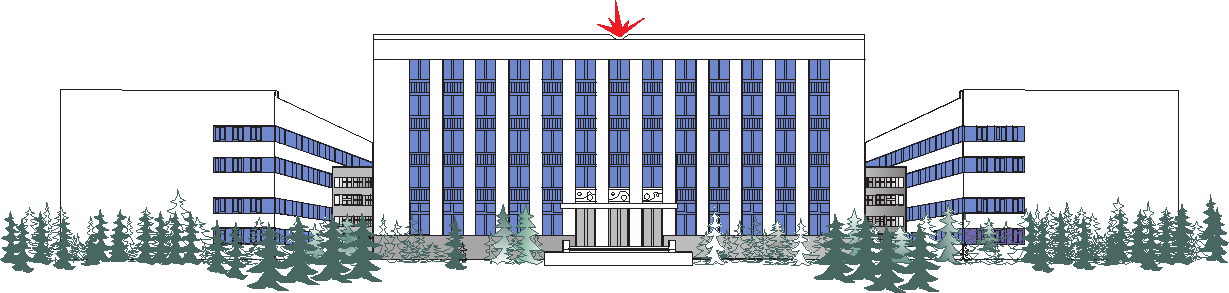
\includegraphics[width=\linewidth]{binpW.pdf}
	\caption{Рисунок с обтеканием. [12] - определяет высоту рисунка в число строк текста и позволяет отбить дополнительное место для рисунков. {r} - положение картинки на странице, можно слева {l} или справа {r}. 
	}
	\label{fig:image4}
\end{wrapfigure}


\lipsum[1-2]

Для рисунков с обтеканием необходим пакет

\verb|\usepackage{wrapfig}%картинки с обтеканием| 

Но вообще картинки с обтеканием лучше не делать.

\section{Изображения с подписями в \LaTeX}

Современные приложения позволяют создавать изображения с текстом, сразу пропущенным через \LaTeX. 

\subsection{matplotlib}
Например в \verb|python| достаточно использовать в модуле \verb|matplotlib| следующую преамбулу:


\begin{minted}{python}
   rc('text', usetex=True)
   rc('font', family='serif')
   rc('text.latex', 
   preamble=r"\usepackage[english,russian]{babel}")
\end{minted}

Это позволит использовать в подписях текст на русском языке, написанный шрифтом с засечками. Также в \verb|matplotlib| можно писать формулы по правилам \LaTeX'а: \verb*|$2+5=7$|
Подробнее:
\begin{itemize}
	\item \href{https://matplotlib.org/stable/tutorials/text/usetex.html?highlight=latex}{https://matplotlib.org/stable/tutorials/text/usetex.html?highlight=latex}
	\item \href{https://pyprog.pro/mpl/mpl_latex_title.html}{https://pyprog.pro/mpl/mpl\_latex\_title.html}
	\item \href{http://s.arboreus.com/2009/04/cyrillic-letters-in-matplotlibpylab.html}{http://s.arboreus.com/2009/04/cyrillic-letters-in-matplotlibpylab.html}
\end{itemize}

\subsection{gnuplot}

Также это можно делать в \verb*|gnuplot|'е: 

\href{http://www.gnuplot.info/docs/tutorial.pdf}{http://www.gnuplot.info/docs/tutorial.pdf}

В самом \LaTeX'е есть возможность строить графики \verb*|gnuplot|'ом с помощью пакета \href{https://mirror.truenetwork.ru/CTAN/macros/latex/contrib/gnuplottex/gnuplottex.pdf}{gnuplottex}.

 Пример использования:  \href{https://habr.com/ru/post/250087/}{https://habr.com/ru/post/250087/}



\chapter{Формулы}\label{ch:eq}
\begin{itemize}
	\item \href{http://mydebianblog.blogspot.com/2009/01/latex-math-in-latex.html}{http://mydebianblog.blogspot.com/2009/01/latex-math-in-latex.html}
\item 	\href{https://www.overleaf.com/learn/latex/mathematical_expressions}{https://www.overleaf.com/learn/latex/mathematical\_expressions}
\end{itemize}

\section{включённые в текст}
Без ограничения общности будем считать, что свет распространяется вдоль координаты $r$. Тогда элемент метрики есть просто $dR = dr/\sqrt{1 - kr^2}$, где $k = 0, +1, -1$ для пространства с нулевой, положительной или отрицательной кривизной, соответственно. Пусть свет был испущен в точке с координатой $r_{em}$ в момент времени $t_{em}$ и принят в точке с координатой $r_{obs} = 0$ в момент времени $t_{obs}$.
\section{вне текста}
Темп  расширения  Вселенной,  т. е.  относительное  увеличение  расстояний  в  единицу  времени,  характеризуется  параметром  Хаббла $$H(t)\equiv\dfrac{\dot{a}(t)}{a(t)}.$$ Параметр  Хаббла  зависит  от  времени;  для  его  современного  значения  применяем, как  обычно,  обозначение  $H_0$.

\begin{gather}\label{f1}
	z=\dfrac{\lambda_{obs}-\lambda_{em}}{\lambda_{em}}\\
	H(t)\equiv\dfrac{\dot{a}(t)}{a(t)}.
\end{gather}

Без нумерации (добавить *)

\begin{gather*}\label{f2}
	z=\dfrac{\lambda_{obs}-\lambda_{em}}{\lambda_{em}}\\
	H(t)\equiv\dfrac{\dot{a}(t)}{a(t)}.
\end{gather*}


С выравниванием (относительно позиции обозначенной \&)
\begin{align}\label{f3}
	\dfrac{\partial\rho}{\partial t}+\nabla(\rho\mathbf{v})&= 0\\
	\dfrac{\partial\mathbf{v}}{\partial t}+(\mathbf{v}\nabla)\mathbf{v}&=-\dfrac{1}{\rho}\nabla P-\nabla\psi\\
	\dfrac{d}{dt}\left(\dfrac{P}{\rho^\gamma}\right)&=0\\
	\nabla^2\psi&=4\pi G\rho
\end{align}

Ссылки на формулы: \ref{f1} и \ref{f2}

Сайты, позволяющие набирать формулы и сразу конвертировать их в изображения (растровые и pdf) (полезно для последующего импорта в PowerPoint презентации):
\begin{itemize}
	\item \href{https://latex.codecogs.com/eqneditor/editor.php}{https://latex.codecogs.com/eqneditor/editor.php} 
	\item \href{https://www.latex4technics.com/}{https://www.latex4technics.com/}
\end{itemize}

Сайт, конвертирующий рукописный ввод в \LaTeX~код:

\href{https://webdemo.myscript.com/views/math/index.html}{https://webdemo.myscript.com/views/math/index.html}
\chapter{Листинги кода}\label{ch:code}

Для включения в текст листингов кода удобно использовать пакет

\verb|\usepackage{minted}|

Для использования нужно будет верстать с ключём \mintinline{sh}{-shell-escape}:
\begin{minted}{c++}
latex -shell-escape doc.tex
\end{minted}

Вместо \mintinline{sh}{latex} может быть \mintinline{sh}{pdflatex} или \mintinline{sh}{xelatex}.

Код, включённый в текст: 

\verb|\mintinline{c++}{float var;}|:

 \mintinline{c}{float var;} 

Или так

\begin{minted}{c++}
vector<Param> All_Parameters;
struct Param
{
   short int Var0;
   float_t Var1;//float_t переменная 
   bool Tr;
   vector<string> Param_Values;//значения параметра
};
\end{minted}


\chapter{Библиография}\label{ch:bib}



В данном шаблоне используется подход к генерированию библиографии с помощью bibtex. Эта система позволяет генерировать список литературы в заданном стиле используя базу данных статей в определённом формате.

\begin{itemize}
	\item \href{https://ru.wikipedia.org/wiki/BibTeX}{https://ru.wikipedia.org/wiki/BibTeX}
	\item  \href{https://www.overleaf.com/learn/latex/Bibliography_management_with_bibtex}{\small https://www.overleaf.com/learn/latex/Bibliography\_management\_with\_bibtex}
	\item \href{http://mydebianblog.blogspot.com/2006/11/latex-jabref.html}{http://mydebianblog.blogspot.com/2006/11/latex-jabref.html}
	\item 	\href{http://www.bibtex.org/Using/}{http://www.bibtex.org/Using/}
	\item \href{https://en.wikibooks.org/wiki/LaTeX/Bibliography_Management}{https://en.wikibooks.org/wiki/LaTeX/Bibliography\_Management}
\end{itemize}

\section{Использование bibtex}

\begin{enumerate}
	\item Либо в преамбуле документа, либо непосредственно перед вызовом команды построения библиографии указать её стиль:  
	
	\verb|\bibliographystyle{Style}|
	
	Здесь \verb|Style| -- стиль. Есть предустановленные:
	
	\href{https://www.overleaf.com/learn/latex/bibtex_bibliography_styles}{https://www.overleaf.com/learn/latex/bibtex\_bibliography\_styles}
	
	Но можно использовать сторонние, указав путь к соответствующему \verb|.bst| файлу.
	\item В тексте ссылка на литературу указывается с помощью команды: 
	
	\verb|\cite{PubName}| (и её вариаций), получается: \cite{Annenkov2020,Annenkov2019,Annenkov2019d}
	\verb|PubName| -- идентификатор статьи, хранящейся в базе данных статей (простой текстовый файл \verb|.bib|)
	
	\item В том месте где мы хотим сгенерировать библиографию вызываем команду:
	
	\verb|\bibliography{RefSource}|
	
	Здесь \verb|RefSource| -- адрес  \verb|.bib| файла с базой литературы. Записи в нём хранятся в виде:
	
\begin{small}
	\begin{minted}{bibtex}
@article{Annenkov2020,
author = {Annenkov, V. V. and Volchok, E. P. and 
Timofeev, I. V.},
doi = {10.3847/1538-4357/abbef2},
issn = {15384357},
journal = {The Astrophysical Journal},
month = {nov},
number = {2},
pages = {88},
title = {{Electromagnetic Emission Produced by 
Three-wave Interactions in a Plasma with 
Continuously Injected Counterstreaming Electron Beams}},
url = {https://iopscience.iop.org/article/10.3847/
1538-4357/abbef2},
volume = {904},
year = {2020}
}
	\end{minted}
\end{small}

Здесь \verb|Annenkov2020|~--- идентификатор публикации. Как правило, с сайтов журналов можно брать информацию о статьях сразу в таком формате.

\item  Последовательно применить к документу команды:

\begin{minted}{sh}
latex doc.tex
latex doc.tex
bibtex doc.tex
latex doc.tex
\end{minted}

Здесь вместо \mintinline{sh}{latex} может быть любая другая команда обработки \mintinline{sh}{.tex} файла (\mintinline{sh}{pdflatex, xelatex ....}). 

Зачастую IDE сами по нажатию одной кнопки проделывают всё это.
\end{enumerate}

\section{Поддержка базы данных статей}

Базу данных публикаций в формате bibtex'а можно наполнять и поддерживать с помощью разных инструментов:

\begin{enumerate}
	\item JabRef \href{https://www.jabref.org/}{https://www.jabref.org/} 
	\item Zotero \href{https://www.zotero.org/}{https://www.zotero.org/}
	\item Mendeley \href{https://www.mendeley.com/}{https://www.mendeley.com/}
\end{enumerate}

Эти системы позволяют в удобной форме хранить и обрабатывать информацию о публикациях. Импортировать её с сайтов, pdf файлов статей и т.п.

Последние две системы также хранят всю базу в облаке.






\chapter{Tikz}\label{ch:tikz}


Пакет Tikz позволяет создавать средствами \LaTeX~разного рода рисунки и диаграммы (простые и очень сложные). В большей степени актуально для \href{https://ru.overleaf.com/learn/latex/Posters}{постеров}/презентаций, но и в текстах может пригодиться.


Пример диаграммы, построенной средствами Tikz:


\begin{small}
	\begin{minipage}[t]{1\linewidth}
	\hspace*{-0.1\linewidth}
	\begin{tikzpicture}[]
		\node[xshift=3.5cm] at (0,0) (1) {Естественные науки};
		\node [below right  = 2cm and 4cm of 1] (2) {Информатика};
		\node [below left = 0.9cm and 2 cm  of 1] (1a) {$\ldots$};
		\draw [-{Stealth[length=3mm]}] (1) -- (1a);
		\node [below left = 0.7cm and -1 cm  of 1] (3) {Физика};
		\draw [-{Stealth[length=3mm]}] (1) -- (3);
		\node [right  = 1cm  of 3] (4) {Химия};
		\node [below left= 0.5 cm and 0.5cm of 4] (4a) {$\ldots$};
		\draw [-{Stealth[length=3mm]}] (4) -- (4a);
		\draw [-{Stealth[length=3mm]}] (1) -- (4);
		\node [right  = 1cm  of 4] (5) {Биология};
		\node [below = 0.8 cm of 5] (5a) {$\ldots$};
		\draw [-{Stealth[length=3mm]}] (5) -- (5a);
		\draw [-{Stealth[length=3mm]}] (1) -- (5);
		
		\node [below right  = -1.8cm and 1.cm  of 5] (5a) {Биоинформатика};
		\node [below   = 1cm of 2] (2a) {$\ldots$};
		\draw [-{Stealth[length=3mm]}] (2) -- (2a); 
		\draw [-{Stealth[length=3mm]}] (2) -- (5a); 
		\draw [-{Stealth[length=3mm]}] (5) -- (5a);
		\node [below left = 0.5 cm and 1. cm of 3] (6) {$\bullet$ Механика};
		\draw [-{Stealth[length=3mm]}] (3) -- (6);
		\node [below = 0.1cm of 6](7) {$\bullet$ Квантовая физика };
		\node [below = 0.1cm of 7](8) {$\bullet$ Электродинамика};
		\node [below = 0.1cm of 8](9) {$\bullet$ Оптика};
		\node [below = 0.1cm of 9](10) {$\bullet$ Термодинамика};
		\node [below = 0.1cm of 10](11) {$\bullet$ Статистическая физика};
		\node [below = 0.1cm of 11](12) {$\ldots$};
		
		\node [below right= 1.5 cm and 0. cm of 3,rectangle,draw] (p0) {\textbf{Физика плазмы}}; 
		\draw [-{Stealth[length=3mm]}] (6.east) -- (p0.north west);
		\draw [-{Stealth[length=3mm]}] (7.east) -- (p0.west); 
		\draw [-{Stealth[length=3mm]}] (8.east) -- (p0.south west); 
		\draw [-{Stealth[length=3mm]}] (9.east) -- (p0); 
		\draw [-{Stealth[length=3mm]}] (4) -- (p0);
		\draw [-{Stealth[length=3mm]}] (2) -- (p0.east); 
		\draw [-{Stealth[length=3mm]}] (10.east) -- (p0); 
		\draw [-{Stealth[length=3mm]}] (11.east) -- ([xshift=0.2cm]p0.south); 
		
		\node [below right= 1 cm and -1. cm of p0] (p1) {$\bullet$ Физика космической плазмы}; 
		\node [below = 0.1cm of p1](p2) {$\bullet$ Физика холодной плазмы};
		\node [below = 0.1cm of p2](p3) {$\ldots$};
		\node [below = 0.1cm of p3](p4) {$\bullet$ Управляемый термоядерный синтез (УТС)};
		\draw [-{Stealth[length=3mm]}] (p0) -- (p1);
		
		\node [below left= 1.5 cm and 4.5 cm of p4,rectangle,draw] (p41) {\textbf{Открытые ловушки}};     
		\node [right= 0.5 cm of p41] (p42) {Пинчи};     
		\node [right= 0.5 cm of p42] (p43) {Стеллараторы};    
		\node [right= 0.5 cm of p43] (p44) {Инерциальный УТС};   
		\node [right= 0.5 cm of p44,rectangle,draw] (p45) {\textbf{Токамаки}};  
		
		\draw [-{Stealth[length=3mm]}] (p4) -- (p41.north);   
		\draw [-{Stealth[length=3mm]}] (p4) -- (p42.north);
		\draw [-{Stealth[length=3mm]}] (p4) -- (p43.north);   
		\draw [-{Stealth[length=3mm]}] (p4) -- (p44.north);
		\draw [-{Stealth[length=3mm]}] (p4) -- (p45.north);
		\node [below= 0.5 cm of p43] (cap) {Упрощённая структурная схема классификации естественных наук,
		};  
		\node [below = 0 of cap] (cap1) {а также список основных научных программ, направленных на решение проблемы УТС.};       
	\end{tikzpicture}
	\vspace{10pt}
\end{minipage}%


\begin{figure}
	\centering
	\smartdiagram[circular diagram:clockwise]{Edit,
		pdf\LaTeX, Bib\TeX/ biber, make\-index, pdf\LaTeX}
	\caption{''Smart'' диаграммы из пакета  \href{https://texample.net/tikz/examples/feature/smartdiagram/}{smartdiagram}}
\end{figure}

\begin{itemize}
	\item \href{https://ru.wikipedia.org/wiki/PGF/Tikz}{https://ru.wikipedia.org/wiki/PGF/Tikz}
	\item \href{https://www.overleaf.com/learn/latex/TikZ_package}{https://www.overleaf.com/learn/latex/TikZ\_package}
	\item \href{https://texample.net/tikz/examples/}{https://texample.net/tikz/examples/}
	\item \href{https://ctan.org/pkg/tcolorbox}{https://ctan.org/pkg/tcolorbox} -- пакет для построения цветных фреймов
\end{itemize}


\end{small}



%конец глав с примерами

\Conclusion

В заключении (выводе) следует четко сформулировать основные выводы, к которым пришел автор. Выводы должны быть краткими и органически вытекать из содержания работы. Разрешается повторить основные выводы соответствующих глав, но при этом предпочтительнее стремиться сделать некоторые обобщения по результатам проведенного исследования в целом.
%Заключение


\References%вставка библиографии

%Приложения (если вдруг нужны)
\Appendix


Этот элемент структуры работы не является обязательным. Приложения целесообразно вводить, когда автор использует относительно большое количество громоздких таблиц, статистического материала. Такой материал, помещенный в основную часть, затруднил бы чтение работы. Обычно в тексте достаточно лишь сослаться на подобную информацию, включенную в приложение.



\begin{table}[H]
	\caption{Такая таблица по ГОСТу}
	\label{tab:GOST3}
	\begin{center}
		\begin{tabular}{|c|c|c|}
			\hline
			\multirow{3}{*}{Размеры нестандартных болтов} & \multicolumn{2}{c|}{Диаметр} \\
			\cline{2-3}
			& Норма & Разброс \\
			\cline{2-3}
			& 10 мм & 1 мм \\
			\hline
		\end{tabular}
	\end{center}
\end{table}
Ссылка на таблицу в Приложении: Таблица~\ref{tab:GOST3}

\begin{figure}[h]
	\centering
	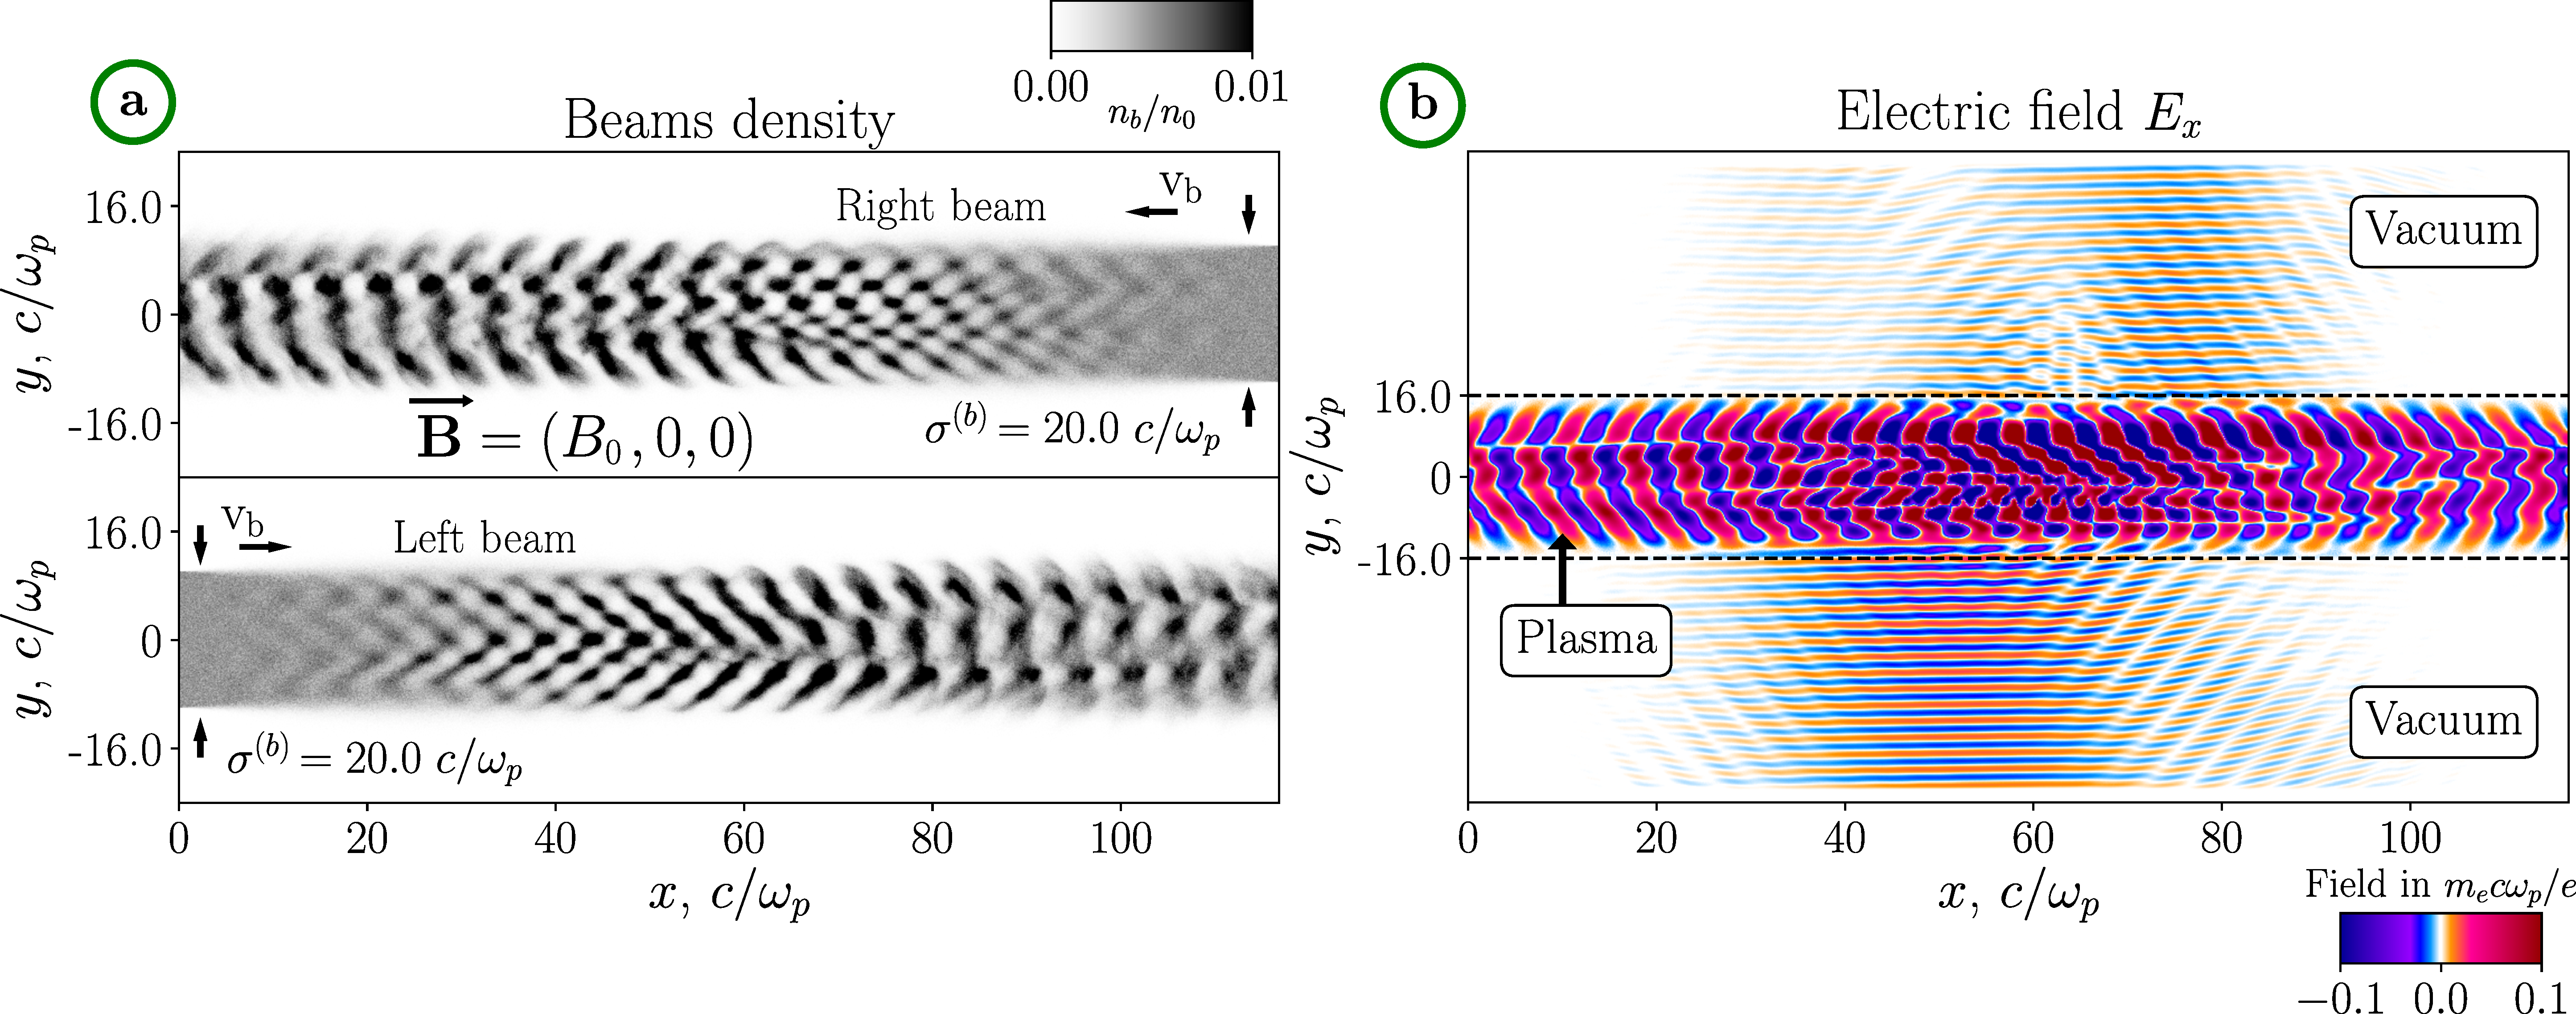
\includegraphics[width=0.45\linewidth]{fig2.pdf}
	\caption{Одна картинка по центру размером 0.45 длины строки}
	\label{fig:App1}%ссылка на картинку
\end{figure}

Ссылка на картинку в Приложении: Рисунок~\ref{fig:App1}


\end{document}